\documentclass[11pt]{article}

\usepackage[T1]{fontenc}
\usepackage{lmodern}
\usepackage{cmap}
\usepackage[a4paper,margin=1in]{geometry}
\usepackage{booktabs}
\usepackage{array}
\usepackage{graphicx}
\usepackage{xurl}
\usepackage{hyperref}
\usepackage{enumitem}
\usepackage{amsmath}
\usepackage{amssymb}
\usepackage{longtable}
\usepackage{tabularx}
\newcolumntype{P}[1]{>{\raggedright\arraybackslash}p{#1}}
\newcolumntype{Y}{>{\raggedright\arraybackslash}X}
\usepackage{tikz}
\usetikzlibrary{positioning,arrows.meta,backgrounds}
\setlength{\emergencystretch}{2em}
\usepackage[backend=bibtex,style=numeric,sorting=none,eprint=true,doi=true,url=true]{biblatex}
\addbibresource{references.bib}

% Document metadata. Kept in sync with paper/witnessability-model/metadata.yaml, which is the
% single source of truth; scripts/qa.py fails the build if the two ever disagree. The title here is
% the unbroken title -- the line break in \title below is a display device, not part of the name.
% Author display form is the founder-decided canonical form for WM 1.1; identity continuity with
% the WM 1.0 artifacts rests on ORCID, not on string equality of display names.
\hypersetup{
  pdftitle={Toward a Witnessability Model for AI and Software Execution Systems},
  pdfauthor={Mikhail A. Sergeev and Vladimir Ikher},
  pdfsubject={AI agents; execution evidence; runtime assurance; AI governance; witnessability; software assurance},
  pdfkeywords={witnessability, AI agents, execution evidence, provenance, attestations, runtime verification}
}

\title{Toward a Witnessability Model for AI\\
and Software Execution Systems\\[0.5em]
\large A Boundary-Based Framework for Classifying Execution Evidence}
\author{Mikhail A. Sergeev\\
Independent Researcher\\
ORCID 0009-0001-6443-855X
\and
Vladimir Ikher\\
Independent Researcher\\
ORCID 0009-0000-0084-704X}
\date{Version 1.1 (bridge revision of the 1.0 line) --- Draft, July 2026}

\begin{document}

\maketitle

\begin{abstract}
Modern AI and software systems increasingly rely on autonomous execution, orchestration frameworks, workflow engines, agent runtimes, tool-calling protocols, serverless execution environments, and governance layers. These systems generate many forms of evidence: logs, traces, metrics, audit records, policy decisions, workflow histories, tool-call records, software attestations, provenance statements, and compliance reports. However, these artifacts often answer different questions and are frequently conflated.

This paper introduces the \emph{Witnessability Model}, a boundary-based framework for classifying the strength of execution-related evidence available for actions performed by software and AI systems. The model distinguishes six execution-evidence levels: observation, intent, invocation, execution, provenance linkage, and independent verification. The paper's central commitment, the Boundary Ceiling (Axiom BC in this revision), bounds the execution-evidence level a witness can honestly claim by the strongest execution-relevant boundary it controls; independent verification qualifies a claim at its captured level rather than raising it.

The paper further proposes a \emph{Witness Boundary Taxonomy} and applies the model to contemporary systems including observability frameworks, CI/CD platforms, workflow engines, AI agent frameworks, tool-calling protocols, automation platforms, serverless runtimes, coding agents, software supply-chain attestation systems, and trusted execution mechanisms.

The analysis suggests that execution ownership, rather than the number of integrations, policies, traces, or attestations, is the primary determinant of attainable witnessability. The model clarifies the distinction between seeing an event, approving an action, invoking a tool, owning execution, linking execution to provenance, and enabling independent verification.

Because these levels carry different evidentiary weight, conflating them creates operational, legal, and governance risk in audit, liability, and AI-governance settings.
\end{abstract}

\noindent\textbf{Keywords:} witnessability, AI agents, execution evidence, provenance, attestations, observability, software supply chain, runtime verification, execution ownership, agent runtimes, AI governance, auditability, operational risk, independent verification, software execution.

\subsection*{Version Identity and Provenance}

This document is \textbf{Version 1.1}, a bridge revision of the Version 1.0 line. Version 1.0 exists as two byte-distinct artifacts; both are superseded by this revision:

\begin{center}
\small
\begin{tabularx}{\textwidth}{@{}Yll@{}}
\toprule
Artifact & SHA-256 & Status \\
\midrule
SSRN deposit (abstract 6994720), ``Version 1.0 $\cdot$ June 2026'', two authors & \texttt{295eb6cb\ldots{}9389d} & canonical 1.0 \\
arXiv-line PDF, ``Preprint --- June 2026'' (v0.5.1 file lineage) & \texttt{f3339324\ldots{}1255e} & secondary 1.0 line \\
\bottomrule
\end{tabularx}
\end{center}

From this revision onward the version number is printed on the title page of every artifact, and each released artifact is identified by its SHA-256 digest. The complete change log against canonical 1.0 accompanies this document (\texttt{CHANGELOG-WM-1.0-to-1.1.md}).

\emph{Scope of this revision.} Version 1.1 stays within the Version 1.0 line: the WL vocabulary and the Boundary Ceiling are retained, with the corrections recorded in the change log (qualified states, axiomatic status of the ceiling, acceptance and composition semantics, migration rules, and the relation to the Witnessability Conceptual Core). A typed reformulation of the model --- replacing the scalar vocabulary entirely --- is reserved for Version 2.0, which will be released only in synchrony with the revision of the Witnessed Execution Protocol that encodes it.

\section{Introduction}

Software systems increasingly act through automated pipelines, workflow engines, AI agents, orchestration platforms, serverless runtimes, and tool-calling frameworks. In many environments, humans no longer execute each action directly. Instead, they define goals, prompts, policies, workflows, permissions, deployment rules, or constraints, while software systems perform actions across chains of components and trust domains.

This shift creates a growing evidence problem. Modern systems can often produce logs, metrics, traces, audit records, policy decisions, tool-call records, workflow histories, execution traces, provenance attestations, software bills of materials, and compliance reports. Yet these artifacts do not all prove the same thing.

A policy system may prove that an action was approved. An observability system may show that a request occurred. A workflow engine may show that a task was scheduled. A supply-chain attestation may prove how an artifact was built. A runtime verification monitor may evaluate whether a trace satisfies a formal property. None of these necessarily proves, by itself, what action actually executed, under which boundary, with which inputs, with which outputs, and with what degree of independent verifiability.

\subsection{Problem Statement}

Evidence artifacts in modern AI and software systems are often conflated under broad terms such as ``auditability,'' ``traceability,'' ``observability,'' ``provenance,'' ``compliance,'' or ``verification.'' This makes it difficult to evaluate what a system can honestly claim about execution.

For example, a governance system may prove that a decision was approved, but not that the approved action executed. An observability platform may record that a request occurred, but not own the execution environment that handled it. A tool-calling protocol may mediate invocation, but not control the tool's internal execution. A supply-chain attestation may link software to its build process, but not prove a later runtime action. A workflow engine may own task scheduling while delegating execution to external services. An AI agent may produce a reasoning trace, but not prove that an externally invoked side effect occurred as claimed.

In institutional settings---audit, liability, AI governance, procurement, and post-incident reconstruction---this ambiguity is itself a source of operational, legal, and governance risk: an organization may be able to show that an action was approved or logged, yet be unable to establish what actually executed, under which boundary, and with what independently verifiable evidence.

\subsection{Research Question}

This paper asks:

\begin{quote}
What execution-evidence levels can be produced by software and AI systems, and what determines the maximum level that can be honestly claimed?
\end{quote}

A secondary question follows:

\begin{quote}
How can systems be classified according to the boundary they control and the resulting ceiling of witnessability?
\end{quote}

\subsection{Contribution}

This paper contributes:

\begin{enumerate}[leftmargin=*]
\item The \emph{Witnessability Model}, which classifies execution-evidence levels from WL0 to WL5.
\item The \emph{Boundary Ceiling} (stated in this revision as Axiom BC), which bounds the honest execution-evidence claim of a witness by the strongest execution-relevant boundary it controls; independent verification qualifies a claim at its captured level rather than raising it (Section~\ref{sec:axiom-bc}).
\item A \emph{Witness Boundary Taxonomy}, distinguishing observation, intent, invocation, execution, provenance, and verification boundaries.
\item A comparative evaluation framework for analyzing observability tools, CI/CD platforms, workflow engines, AI agent frameworks, tool-calling protocols, serverless runtimes, coding agents, and supply-chain attestation systems.
\item A conceptual separation between observability, governance, provenance, runtime verification, and witnessability.
\end{enumerate}

This paper does not claim to introduce runtime evidence, provenance, receipts, or execution tracing as new categories; its contribution is the boundary-based ceiling invariant that constrains the maximum honest execution-evidence claim a witness can make.
It is a conceptual framework rather than a system or implementation: like other vendor-neutral assurance and provenance frameworks, its contribution is definitional and classificatory, and it is intended to be evaluated on those terms.

\subsection{What Is New}

The model is not a claim that common evidence artifacts are new. This paper does not claim that logs are new, that provenance is new, that attestations are new, or that verification is new. It also does not claim that observability, auditability, provenance, or runtime verification are reducible to witnessability.

The claim is narrower. This paper introduces a boundary-based ceiling on execution-evidence claims; a formal distinction between observation, invocation, and execution ownership; and a claim-strength classification that is independent of artifact type. A log, trace, attestation, workflow history, or verification report may support different execution-evidence claims depending on which boundary produced it and which boundary can verify it.

\begin{table}[h]
\centering
\scriptsize
\setlength{\tabcolsep}{3pt}
\renewcommand{\arraystretch}{1.12}
\begin{tabularx}{\textwidth}{@{}P{0.16\textwidth}YYYYY@{}}
\toprule
 & Observability & Auditability & Provenance & Runtime Verification & Witnessability \\
\midrule
Primary question & What can be seen or measured? & Can actions and decisions be reviewed later? & Where did an artifact or result come from? & Does an execution trace satisfy a property? & What execution-evidence claim can a witness honestly support? \\
Evidence type & Logs, metrics, traces, events. & Records, controls, approvals, audit trails. & Source, build, artifact, dependency, or origin links. & Traces plus formal or executable properties. & Boundary-grounded claims about action evidence. \\
Execution ownership required? & No. & No. & Not by itself. & Not by itself. & Required for WL3 execution evidence and above. \\
Independent verification required? & Not inherent. & Sometimes, depending on audit regime. & Often useful for origin claims. & Not inherent; monitors may be internal. & Required for WL5. \\
Honest claim ceiling? & Not defined. & Not defined. & Supports origin/provenance claims, not runtime action by itself. & Evaluates properties over available evidence. & Explicitly defined by the strongest controlled or grounded boundary. Independent verification qualifies a claim; it does not raise the ceiling. \\
\bottomrule
\end{tabularx}
\caption{Witnessability compared with adjacent evidence concepts.}
\end{table}

\subsection{Central Thesis}

The central thesis of this paper is:

\begin{quote}
The maximum strength of an execution-evidence claim is determined not by the number of logs, integrations, policies, traces, or attestations a system produces, but by the execution-relevant boundary controlled by the witness.
\end{quote}

\section{Motivating Examples}

\subsection{Governance Approval Without Execution Proof}
An AI governance layer may evaluate a proposed tool call and record that the action was allowed by policy. This record may be valuable for compliance. It may show intent, authorization, and policy alignment. However, such a record does not prove that the action actually executed.

\subsection{Trace Visibility Without Execution Ownership}
A distributed tracing system may record that a request crossed a service boundary. It may show timing, service identity, latency, status codes, and related spans. However, unless the tracing system controls the execution boundary, the trace remains an observation of behavior rather than proof of owned execution.

\subsection{Tool Invocation Without Tool Execution Proof}
An AI agent may call an external tool through a standardized protocol. The agent runtime may record the tool name, parameters, response, and timestamp. This may prove that an invocation occurred across a controlled boundary. But if the actual tool executes in an external system, the agent runtime may not be able to prove how that tool executed internally.

\subsection{Build Provenance Without Runtime Proof}
A software artifact may have strong build provenance, signed attestations, and verifiable source linkage. This may establish where the artifact came from and how it was built. However, build provenance does not automatically prove that a specific runtime action was later executed by that artifact under a specific environment.

\subsection{Execution Ownership Without Independent Verification}
A workflow engine, serverless runtime, or CI/CD runner may own the execution process. It may capture command, environment, exit code, outputs, and result digests. This can provide strong execution evidence. But if all evidence is produced and stored by the same operator, independent verification may still require additional mechanisms such as signed receipts, transparency logs, reproducible checks, remote attestation, external witnesses, or third-party verification.

\section{Related Work}

\subsection{Observability}
Observability systems collect, process, export, and correlate telemetry such as logs, metrics, traces, events, and resource metadata. OpenTelemetry is a leading vendor-neutral observability framework that supports the generation, collection, and export of telemetry data such as traces, metrics, and logs~\cite{opentelemetry_docs,opentelemetry_what_is}. Observability systems are essential for debugging, monitoring, incident response, performance analysis, and operational visibility.

However, observability is primarily concerned with what can be seen, measured, and correlated. It does not, by itself, define the maximum execution-evidence claim that a system can honestly make.

\subsection{Runtime Verification}
Runtime verification studies the dynamic analysis of execution traces against formal specifications~\cite{sanchez_runtime_verification,weil_runtime_interactions_2025}. It typically involves instrumentation, trace generation, monitor synthesis, and the evaluation of traces against generated monitors or formalized requirements.

Witnessability addresses a different but complementary question. Runtime verification asks whether an execution satisfies a specified property. Witnessability asks what kind of execution-related evidence exists before a domain-specific property is evaluated.

\paragraph{Terminology: witnessability.} The term \emph{witnessability} has prior use in programming languages and formal methods, notably in Ding and Zhang's work on the witnessability of undecidable problems~\cite{DingZhang2023}, where it concerns undecidable problems and their decidable approximations. Our use is distinct and operational: we use \emph{witnessability} to refer to the strength of execution-evidence claims a witness can honestly support about runtime actions, given the boundary it controls.

\subsection{Provenance Models, Attestation Architectures, and Transparency}
The W3C PROV data model standardizes the vocabulary of provenance graphs (entities, activities, agents, derivations)~\cite{w3c_prov}; the PROV qualifier of this model is unrelated to it in mechanism --- it marks a bound origin linkage for an executed action, not a graph vocabulary --- and profiles realizing provenance evidence may well serialize it in PROV terms. The IETF RATS architecture~\cite{rfc9334_rats} standardizes remote attestation roles (attester, verifier, relying party) whose appraisal concerns environment identity and integrity; SCITT~\cite{rfc9943_scitt} standardizes transparency services over signed statements. Both are boundary substrates for this model: attestation can ground an execution boundary, and transparency receipts can carry custody evidence, but neither by itself establishes the action-level content of a claim.

Closest in intent among 2026 work are the evidentiary-adequacy criterion for agentic AI oversight~\cite{evidentiary_adequacy_2026}, which asks when runtime records suffice for legal findings and shares this model's refusal to treat record volume as evidence strength, and graduated evidence-maturity schemes such as the Decision Evidence Maturity Model~\cite{demm_2026}. The present model differs from maturity schemes on the same ground it differs from its own Version 1.0 ladder: content depth and independent verifiability are typed dimensions, not rungs of one scale.

\paragraph{Terminology: witness.} Beyond the POPL sense of \emph{witnessability} discussed above, the bare word \emph{witness} carries established meanings that this model does not use: the in-toto \emph{Witness} attestation tool, witness cosigning of transparency logs, the cryptographic witness of an NP relation, and blockchain witness nodes. This model prefers the full terms \emph{witnessability level} and \emph{witness boundary}.

\subsection{Software Supply-Chain Security}
Software supply-chain security frameworks such as SLSA, in-toto, and Sigstore focus on artifact integrity, build provenance, signing, identity, and attestations. SLSA defines provenance as verifiable information about where, when, and how a software artifact was produced~\cite{slsa_provenance,slsa_verifying_artifacts}. The in-toto Attestation Framework provides a specification for generating verifiable claims about aspects of how software is produced~\cite{intoto_attestation,intoto_slsa_blog}. GitHub Actions artifact attestations establish build provenance for binaries and container images~\cite{github_actions_attestations,github_actions_attest_concepts}.

These systems are highly relevant to WL4 of the Witnessability Model, where runtime execution is linked to verifiable origin, source, build, artifact, configuration, or deployment materials. However, build-time provenance and runtime execution evidence are not identical.

\subsection{Runtime Governance and Constitutional Frameworks}
Adjacent governance architectures address authorization, constitutional constraints, delegation, and audit reconstructability for deployed AI systems. Sergeev~\cite{sergeev_pai_cd_2026} proposes a constitutional governance framework and identifies the absence of standardized, provider-independent verification infrastructure as an open limitation. Tallam~\cite{tallam_five_plane_2026} presents a runtime governance architecture organized around composite principals and an audit substrate for evidence reconstructability. These frameworks are complementary to the present work: they govern or reconstruct what agents may do, whereas the Witnessability Model addresses what can be proven about what they did---the execution-evidence level a witness can honestly support, bounded by the boundary it controls, independent of the trust tier of the record source.

\subsection{Agent Provenance and Execution Tracing}
Recent work on LLM-agent provenance studies how agent executions can be traced through tool calls, retrieved evidence, memory, intermediate claims, observations, actions, and final answers. Wang et al. provide a systematic review and conceptual framework for evidence tracing and execution provenance in LLM agents~\cite{wang_agent_traces_2026}. Other work explores structured reasoning provenance for autonomous AI agents~\cite{vispute_reasoning_provenance_2026}, dynamic agent observability~\cite{agenttrace_2026}, bounding LLM agents via execution provenance~\cite{agent_sentry_2026}, aligning authorization with execution provenance~\cite{authgraph_2026}, and intent-to-execution integrity~\cite{intent_execution_integrity_2026}.

This work is directly adjacent to witnessability. It addresses how agent behavior unfolds and how evidence supports outputs or actions. The Witnessability Model adds a boundary-based claim ceiling: it asks what level of execution-related claim can honestly be made given the boundary controlled by the witness.

\begin{table}[h]
\centering
\small
\setlength{\tabcolsep}{4pt}
\begin{tabularx}{\textwidth}{@{}P{0.18\textwidth}Y P{0.17\textwidth}P{0.18\textwidth}@{}}
\toprule
Work & Primary contribution & Explicit boundary-ceiling model? & Separates observe / invoke / execute? \\
\midrule
Wang et al.~\cite{wang_agent_traces_2026} & Systematic review of evidence tracing / execution provenance in LLM agents & Partial & Partial \\
Vispute~\cite{vispute_reasoning_provenance_2026} & Structured reasoning provenance & Not explicit & No \\
AuthGraph~\cite{authgraph_2026} & Aligns authorization with execution provenance & Not primary focus & Partial \\
Sequeira et al.~\cite{agent_sentry_2026} & Runtime defense that bounds benign agent execution using action-sequence structure, function-argument provenance, allowlist checks, and an LLM judge & Not primary focus & Partial \\
Witnessability Model (this work) & Boundary-based ceiling on the level of execution-evidence claim & Yes (Boundary Ceiling, WL0--WL5) & Yes \\
\bottomrule
\end{tabularx}
\caption{Agent-provenance / execution-tracing work compared with the Witnessability Model.}
\end{table}

\subsection{Signed Agent Receipts and an Emerging Evidence Industry}
A nascent line of work focuses specifically on signed, independently checkable records of individual agent actions. Figuera's \emph{Notarized Agents} proposes receiver-attested, confidential receipts for AI-agent actions, in which the receiving party co-signs the evidence and a witness-cosigned log records the interaction under an adversary model that admits compromise of both the agent and its operator~\cite{figuera_notarized_agents_2026}. Cordon introduces semantic transactions for tool-using LLM agents, bounding tool execution within transactional units so that an agent's externally visible effects can be scoped, committed, or rolled back~\cite{cordon_semantic_transactions_2026}. Alongside such academic efforts, practitioner and industry work is beginning to explore agent receipts, signed attestations, and execution-evidence records for per-action accountability of autonomous systems. This activity is directly adjacent to witnessability: each effort strengthens the integrity, confidentiality, or scoping of per-action records. The Witnessability Model is complementary rather than competing: it does not propose another receipt format but classifies, for any such record, the execution-evidence level that the producing boundary can honestly support.

\subsection{Workflow, Durable Execution, and Replay}
Workflow engines orchestrate long-running processes, retries, state transitions, and activity execution. Temporal documents workflow event histories and durable execution through replay mechanisms~\cite{temporal_event_history,temporal_durable_execution}. LangGraph provides persistence through checkpoints, enabling state snapshots, replay, human-in-the-loop workflows, time travel debugging, and fault-tolerant execution~\cite{langgraph_persistence,langgraph_time_travel}. Airflow defines tasks as units of execution arranged in DAGs and executed through configured executors~\cite{airflow_tasks,airflow_executor}.

These systems may produce histories that are stronger than ordinary logs, especially when they own scheduling and activity execution. However, workflow witnessability depends on the boundary actually controlled by the workflow system.

\subsection{Tool-Calling Protocols and Agent SDKs}
The Model Context Protocol is an open standard for connecting AI applications to external systems, data sources, tools, and workflows~\cite{mcp_intro,anthropic_mcp}. OpenAI's Agents SDK includes built-in tracing of LLM generations, tool calls, handoffs, guardrails, and custom events~\cite{openai_agents_tracing}. AutoGen is a framework for multi-agent AI applications that can act autonomously or with humans~\cite{autogen_repo,autogen_agent_chat}.

These frameworks are important because they often blur planning, invocation, tool execution, and observation. Their witnessability depends on whether they only orchestrate invocations or also own the execution boundary.

\subsection{Execution-Grounded Coding Agents}
OpenHands describes software agents that interact with developer environments by writing code, using command lines, browsing, and executing code in sandboxed environments~\cite{openhands_platform_2024,openhands_sdk_2025}. AgentForge introduces execution-grounded verification through mandatory sandboxed execution before code propagation~\cite{agentforge_2026}. These systems demonstrate the increasing importance of controlled execution boundaries in AI-assisted software engineering.

\subsection{Serverless, Isolates, and Trusted Execution}
Cloudflare Workers run code in V8 isolates and document a security model based on tenant isolation using V8 isolates rather than conventional processes or VMs~\cite{cloudflare_workers_how,cloudflare_workers_security}. Trusted execution environments and remote attestation may strengthen witnessability by providing externally verifiable claims about execution environment identity and integrity~\cite{attestable_builds_2025,zk_compilation_2026,evidence_ci_2026}. However, attestation of the environment must still be connected to action-level evidence.

\section{Definitions}

\paragraph{Witness.} A witness is a system, component, runtime, service, process, organization, or verifier that records or verifies evidence about an action.

\paragraph{Action.} An action is an operation performed by a software or AI system that changes state, produces output, invokes a tool, calls an API, executes code, modifies data, sends a message, deploys an artifact, or otherwise affects an environment.

\paragraph{Evidence artifact.} An evidence artifact is any record or object used to support a claim about an action.

\paragraph{Boundary.} A boundary is a control surface across which an action is observed, approved, invoked, executed, linked to provenance, or verified.

\paragraph{Execution ownership.} Execution ownership is the capability to run, constrain, capture, or mediate the actual execution of an action within a controlled runtime, process, worker, activity, container, isolate, virtual machine, sandbox, or equivalent execution environment.

Operationally, execution ownership is present when the witness can satisfy most of the following criteria for the action being claimed:
\begin{enumerate}[leftmargin=*]
\item initiate or authorize the execution within a controlled runtime;
\item constrain execution through policy, sandboxing, scheduling, resource limits, or equivalent controls;
\item observe execution internals rather than only boundary-crossing events;
\item bind outputs, exit status, side effects, or result digests to the runtime that produced them; and
\item preserve execution evidence with sufficient integrity to support later reconstruction.
\end{enumerate}

A witness need not satisfy every criterion in every deployment, but a claim of execution ownership becomes weak when most of these capabilities are absent.

\paragraph{Grounded.} A record is \emph{grounded} on a boundary when bound evidence establishes the identity of that boundary and its connection to the claimed action, assessable under the applicable evaluation profile. Grounding decides whether a record may rely on a boundary attested by another party; an ungrounded boundary designation is an attributed self-description of the witness.

\paragraph{Binding.} \emph{Binding evidence} connects records to one another (or a record to its action) such that the connection is itself assessable. Binding is a precondition of composition (Section~\ref{sec:composition}); without it, segment records are individually assessable but their concatenation supports no claim about the whole.

\paragraph{Witnessability.} Witnessability is the maximum strength of an execution-related evidence claim that a witness can honestly make, given the boundary it controls and the verification mechanisms available. This model is an execution-class specialization of the claim-relative notion defined by the Witnessability Conceptual Core~\cite{wcc_core_2026} (Section~\ref{sec:wcc-relation}).

\subsection{System Ceiling and Event Level}
The Witnessability Model defines six execution-evidence levels, denoted WL0--WL5.

A system has a \emph{witnessability ceiling}: the maximum level it can generally support under its architecture and controlled boundary. A specific event has an \emph{achieved execution-evidence level}: the level actually supported by the evidence captured for that event. A system may have a WL3 ceiling while a specific event only achieves WL1 if execution results were not captured.

\subsection{Claim Grammar}
A complete execution-evidence claim may be represented as:

\begin{quote}
Witness $W$ claims that Actor $A$ performed or attempted Action $X$ under Boundary $B$ at Time $T$ with Input $I$, producing Output $O$, under Environment $E$, linked to Origin/Provenance $P$, and verifiable by Verifier $V$, under Trust Assumptions $S$.
\end{quote}

Different execution-evidence levels correspond to different subsets of this claim being supportable.

\begin{table}[h]
\centering
\small
\setlength{\tabcolsep}{4pt}
\begin{tabularx}{\textwidth}{@{}P{0.09\textwidth}Y@{}}
\toprule
Level & Honestly supportable subset of the claim grammar \\
\midrule
WL0 & Actor $A$, Action $X$, Time $T$ as \emph{observed} (observation boundary). \\
WL1 & Adds intent / authority for $X$ (intent / policy boundary). \\
WL2 & Adds Input $I$ across a controlled invocation boundary $B$. \\
WL3 & Adds Output $O$ and Environment $E$ under an owned execution boundary $B$. \\
WL4 & Adds Origin / Provenance $P$. \\
WL5 & Adds an independent Verifier $V$; weakens reliance on Trust Assumptions $S$. \\
\bottomrule
\end{tabularx}
\caption{Claim-grammar subsets honestly supportable at each execution-evidence level. Levels WL0--WL3 are cumulative with the levels below them; WL4 and WL5 are \emph{qualified states} over WL3 --- display labels for provenance linkage and independent verifiability respectively --- not further rungs of a single ladder (Section~\ref{sec:qualified-states}).}
\end{table}

\begin{figure}[t]
\centering
\resizebox{\textwidth}{!}{%
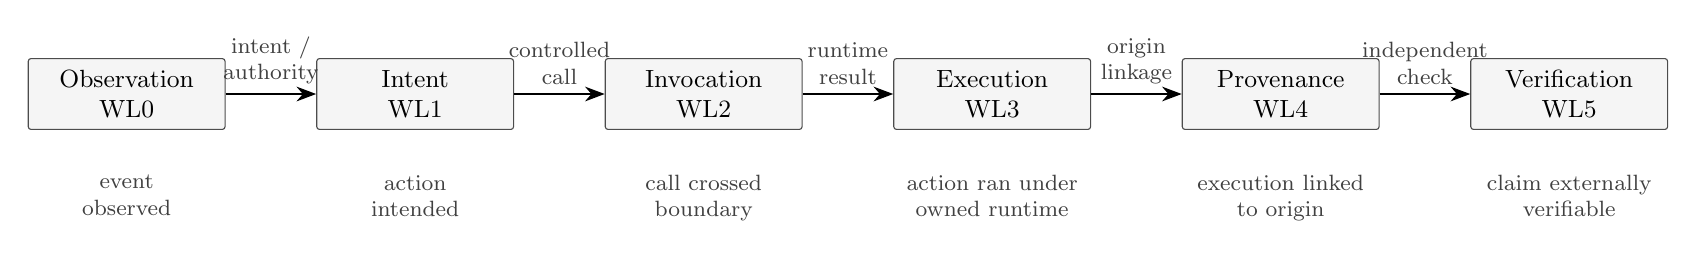
\begin{tikzpicture}[
  font=\small,
  node distance=1.15cm,
  stage/.style={draw=black!70, rounded corners=1pt, minimum width=2.5cm, minimum height=0.9cm, align=center, fill=black!4},
  arrow/.style={-{Stealth[length=2.5mm]}, line width=0.5pt},
  claim/.style={font=\footnotesize, align=center, text=black!75}
]
\node[stage] (obs) {Observation\\WL0};
\node[stage, right=of obs] (intent) {Intent\\WL1};
\node[stage, right=of intent] (invoke) {Invocation\\WL2};
\node[stage, right=of invoke] (exec) {Execution\\WL3};
\node[stage, right=of exec] (prov) {Provenance\\WL4};
\node[stage, right=of prov] (verify) {Verification\\WL5};
\draw[arrow] (obs) -- node[claim, above] {intent /\\authority} (intent);
\draw[arrow] (intent) -- node[claim, above] {controlled\\call} (invoke);
\draw[arrow] (invoke) -- node[claim, above] {runtime\\result} (exec);
\draw[arrow] (exec) -- node[claim, above] {origin\\linkage} (prov);
\draw[arrow] (prov) -- node[claim, above] {independent\\check} (verify);
\node[claim, below=0.45cm of obs] {event\\observed};
\node[claim, below=0.45cm of intent] {action\\intended};
\node[claim, below=0.45cm of invoke] {call crossed\\boundary};
\node[claim, below=0.45cm of exec] {action ran under\\owned runtime};
\node[claim, below=0.45cm of prov] {execution linked\\to origin};
\node[claim, below=0.45cm of verify] {claim externally\\verifiable};
\end{tikzpicture}
}
\caption{Evidence path from observation to independent verification. Each transition adds a new supportable claim only when the witness controls the corresponding boundary, or has grounded its record on it.}
\label{fig:evidence-path}
\end{figure}

\section{The Witnessability Model}

Figure~\ref{fig:boundary-ceiling} summarizes the model: the cumulative content levels WL0--WL3, the qualified states labeled WL4 and WL5 (Section~\ref{sec:qualified-states}), and the Boundary Ceiling bounding the highest claim a witness can honestly make.

\begin{figure}[t]
\centering
\resizebox{\textwidth}{!}{%
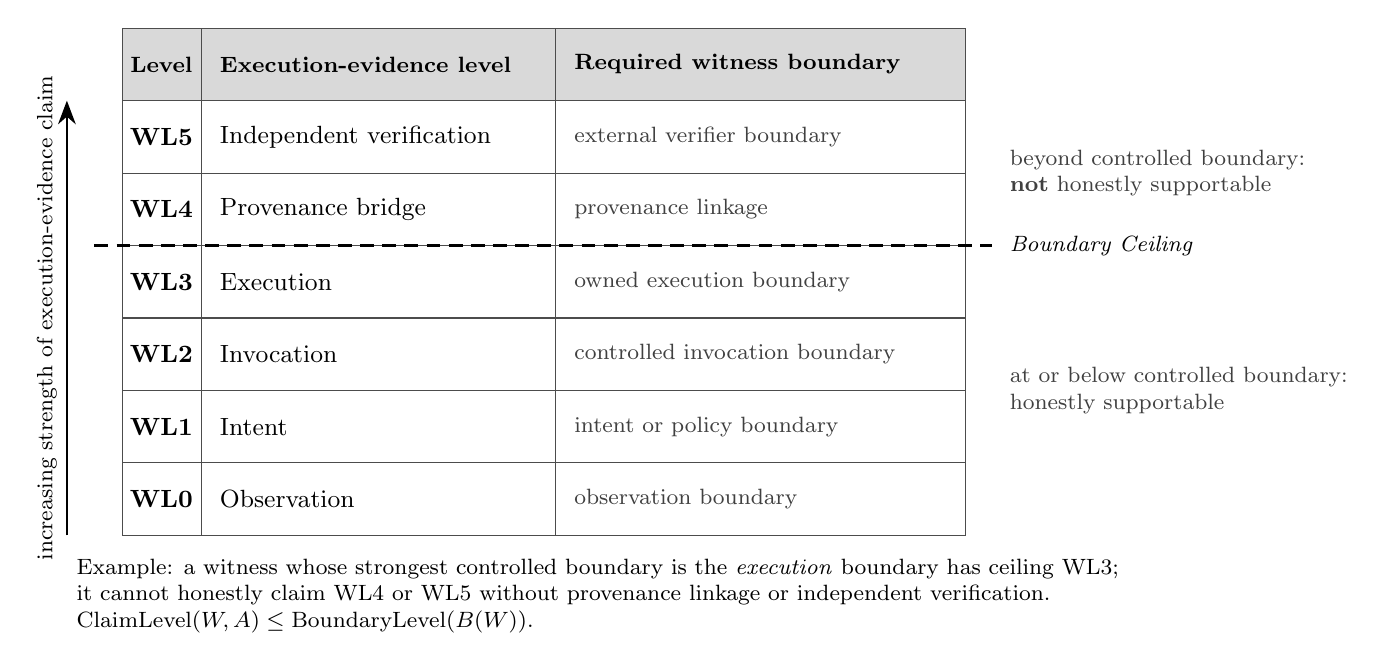
\begin{tikzpicture}[font=\small,
  lvl/.style={draw=black!70, line width=0.4pt, minimum height=0.92cm, anchor=west}]
  \def\x{0}\def\wn{1.0}\def\wname{4.5}\def\wb{5.2}\def\hh{0.92}
  \pgfmathsetmacro{\wtot}{\wn+\wname+\wb}
  \pgfmathsetmacro{\yb}{-\hh/2}
  \pgfmathsetmacro{\yt}{5*\hh+\hh/2}
  \pgfmathsetmacro{\yc}{3*\hh+\hh/2}
  \begin{scope}[on background layer]
    \fill[black!6]  (\x,\yb) rectangle (\x+\wtot,\yc);
    \fill[black!16] (\x,\yc) rectangle (\x+\wtot,\yt);
  \end{scope}
  \foreach \i/\lvl/\name/\bound in {%
    0/WL0/Observation/observation boundary,
    1/WL1/Intent/intent or policy boundary,
    2/WL2/Invocation/controlled invocation boundary,
    3/WL3/Execution/owned execution boundary,
    4/WL4/Provenance bridge/provenance linkage,
    5/WL5/Independent verification/external verifier boundary}{
      \pgfmathsetmacro{\yy}{\i*\hh}
      \node[lvl, minimum width=\wn cm, fill=white] at (\x,\yy) {};
      \node[font=\bfseries\small] at ([xshift=\wn*0.5 cm]\x,\yy) {\lvl};
      \node[lvl, minimum width=\wname cm, fill=white] at (\x+\wn,\yy) {};
      \node[anchor=west, font=\small] at ([xshift=0.12cm]\x+\wn,\yy) {\name};
      \node[lvl, minimum width=\wb cm, fill=white] at (\x+\wn+\wname,\yy) {};
      \node[anchor=west, text=black!75, font=\footnotesize] at ([xshift=0.12cm]\x+\wn+\wname,\yy) {\bound};
  }
  \pgfmathsetmacro{\yhr}{6*\hh}
  \node[lvl, minimum width=\wn cm,    fill=black!15] at (\x,\yhr) {};
  \node[lvl, minimum width=\wname cm, fill=black!15] at (\x+\wn,\yhr) {};
  \node[lvl, minimum width=\wb cm,    fill=black!15] at (\x+\wn+\wname,\yhr) {};
  \node[font=\bfseries\footnotesize] at ([xshift=\wn*0.5 cm]\x,\yhr) {Level};
  \node[anchor=west, font=\bfseries\footnotesize] at ([xshift=0.12cm]\x+\wn,\yhr) {Execution-evidence level};
  \node[anchor=west, font=\bfseries\footnotesize] at ([xshift=0.12cm]\x+\wn+\wname,\yhr) {Required witness boundary};
  \draw[line width=1.1pt, dash pattern=on 5pt off 3pt] (\x-0.35,\yc) -- (\x+\wtot+0.35,\yc);
  \node[anchor=west, font=\footnotesize\itshape] at (\x+\wtot+0.45,\yc) {Boundary Ceiling};
  \pgfmathsetmacro{\yup}{(\yc+\yt)/2}
  \pgfmathsetmacro{\ylo}{(\yb+\yc)/2}
  \node[anchor=west, align=left, font=\footnotesize, text=black!75] at (\x+\wtot+0.45,\yup) {beyond controlled boundary:\\\textbf{not} honestly supportable};
  \node[anchor=west, align=left, font=\footnotesize, text=black!75] at (\x+\wtot+0.45,\ylo) {at or below controlled boundary:\\honestly supportable};
  \draw[-{Stealth[length=3mm]}, line width=0.8pt] (\x-0.7,\yb) -- (\x-0.7,\yt) node[midway, rotate=90, anchor=south, font=\footnotesize] {increasing strength of execution-evidence claim};
  \node[anchor=north west, align=left, font=\footnotesize] at (\x-0.7,\yb-0.18) {Example: a witness whose strongest controlled boundary is the \emph{execution} boundary has ceiling $\mathrm{WL3}$;\\it cannot honestly claim $\mathrm{WL4}$ or $\mathrm{WL5}$ without provenance linkage or independent verification.\\$\mathrm{ClaimLevel}(W,A) \le \mathrm{BoundaryLevel}(B(W))$.};
\end{tikzpicture}
}
\caption{The Witnessability Model. Content levels WL0--WL3 are cumulative, each requiring control of a corresponding witness boundary; the rows labeled WL4 and WL5 are qualified states over WL3 (Section~\ref{sec:qualified-states}), drawn on the ladder for continuity with Version 1.0 display conventions. A witness's Boundary Ceiling is the highest content level supported by the strongest boundary it controls; honest claims lie at or below this ceiling. The dashed line shows an example ceiling for a witness that owns the execution boundary (WL3).}
\label{fig:boundary-ceiling}
\end{figure}

\begin{table}[h]
\centering
\small
\begin{tabularx}{\textwidth}{@{}P{0.08\textwidth}P{0.20\textwidth}Y Y@{}}
\toprule
Level & Name & Core claim & Boundary requirement \\
\midrule
WL0 & Observation & An event was observed or reported. & No execution ownership required. \\
WL1 & Intent & An intended or approved action was recorded. & Control over plan/policy/approval. \\
WL2 & Invocation & A call crossed a controlled invocation boundary. & Control over API/tool/protocol boundary. \\
WL3 & Execution & The action executed under a controlled boundary. & Control over process/activity/runtime. \\
WL4 & Provenance Bridge & Execution is linked to verifiable origin. & WL3 plus provenance linkage. \\
WL5 & Independent Verification & The evidence claim can be verified independently. & External verifier or equivalent mechanism. \\
\bottomrule
\end{tabularx}
\caption{Execution-evidence levels in the Witnessability Model.}
\end{table}

\paragraph{Levels are boundaries, not maturity.} An execution-evidence level is not a maturity, quality, or trust ranking: a higher WL reflects control of a stronger execution-relevant boundary, not a more mature, more secure, or otherwise better system. A WL2 record produced by a system that only mediates invocation is not inferior engineering, and a WL5 claim is not an endorsement of the witness beyond the specific evidence that is independently verified.

\subsection{WL0: Observation}
WL0 evidence records that something was observed or reported. It does not prove intent, invocation mediation, execution ownership, provenance linkage, or independent verification.

\subsection{WL1: Intent}
WL1 evidence records intended, planned, approved, or policy-evaluated action. It proves intent or decision, not necessarily invocation or execution.

\subsection{WL2: Invocation}
WL2 evidence records that an invocation crossed a controlled boundary. It proves controlled invocation, but not necessarily internal execution of the target system.

\subsection{WL3: Execution}
WL3 evidence records that the action executed under a controlled execution boundary. It requires execution ownership.

\subsection{WL4: Provenance Bridge}
WL4 evidence links execution to verifiable origin, such as source commits, build attestations, deployment manifests, artifact digests, SBOMs, or signed configuration records.

\subsection{WL5: Independent Verification}
WL5 evidence allows a third party to verify the evidence claim without relying solely on the original operator. WL5 does not necessarily require deterministic replay of the entire execution. Instead, it requires independent verification of the specific evidence claim being made.

WL5 can be realized through different verification mechanisms that differ in their underlying trust assumptions. A transparency log or public ledger provides independent verification by recording evidence in an append-only structure auditable by third parties, shifting trust to the integrity of the log and its witnesses. A trusted execution environment with remote attestation lets a verifier confirm that evidence was produced inside a measured environment, shifting trust to a hardware root of trust and the attestation chain. A zero-knowledge proof lets a verifier check the validity of a claim while revealing minimal underlying information, shifting trust primarily to cryptographic assumptions. These mechanisms are not mutually exclusive and may be combined; they represent a spectrum of trust assumptions rather than a strict ordering, and the appropriate choice depends on the claim, the adversary model, and applicable privacy constraints.

These mechanisms support a WL5 claim only for the specific claim they independently verify; they do not automatically raise an observation or invocation record to execution evidence.

\subsection{Qualified States, Display Labels, and Ordering}
\label{sec:qualified-states}

Version 1.0 described WL4 and WL5 both as rungs of a cumulative ladder (Table~3, Figure~\ref{fig:boundary-ceiling}) and as qualifications applicable ``to a claim at any lower level'' whose verification ``does not raise the captured level'' (Section 5.6 and the corollaries). These two readings are inconsistent, and downstream protocol work exposed the inconsistency. This revision resolves it \emph{in favor of the qualification reading}, which Version 1.0's own corollaries already entailed.

\paragraph{Content levels and qualifiers.} The content levels form the cumulative chain
\[
\mathrm{WL0} < \mathrm{WL1} < \mathrm{WL2} < \mathrm{WL3},
\]
ordered by executional depth. Independently of content level, a claim may carry \emph{qualifiers}:
\begin{itemize}[leftmargin=*]
\item \textbf{PROV} --- the claimed action is linked to verifiable origin by a bound provenance artifact;
\item \textbf{IV} --- the specific claim is independently verifiable by a non-participant.
\end{itemize}
A witnessability state is a pair $(\ell, Q)$ with $\ell \in \{\mathrm{WL0},\ldots,\mathrm{WL3}\}$ and $Q \subseteq \{\mathrm{PROV}, \mathrm{IV}\}$. IV may attach at any content level; PROV presupposes an executed action and therefore attaches at WL3. Qualifiers never raise the content level.

\paragraph{Display labels.} For continuity, the scalar labels of Version 1.0 are retained as \emph{display labels} for specific states: ``WL4'' displays $(\mathrm{WL3}, \{\mathrm{PROV}\})$ and ``WL5'' displays $(\mathrm{WL3}, \{\mathrm{IV}\})$. Each state has exactly one canonical display: states without a scalar label are displayed as $\mathrm{WL}n[\mathrm{PROV}]$, $\mathrm{WL}n[\mathrm{IV}]$, or $\mathrm{WL3}[\mathrm{PROV},\mathrm{IV}]$; in particular the top state $(\mathrm{WL3},\{\mathrm{PROV},\mathrm{IV}\})$ has no bare scalar label. A bare scalar above WL3 is never used as a sort key.

\paragraph{Ordering.} States are compared componentwise:
\[
(\ell, Q) \le (\ell', Q') \iff \ell \le \ell' \ \wedge\ Q \subseteq Q'.
\]
This is a partial order; in particular $(\mathrm{WL3},\{\mathrm{PROV}\})$ and $(\mathrm{WL3},\{\mathrm{IV}\})$ --- ``WL4'' and ``WL5'' --- are \emph{incomparable}. Any totally ordered presentation of the six labels, including the ladder figures of this paper, is a \emph{display projection}: a profile-defined, justified projection of the partial order in the sense of the Conceptual Core's invariant W-I7 (preserved incomparability)~\cite{wcc_core_2026}. A projection may be used for presentation and for backward-compatible encodings; it must not be used for verdict arithmetic (Section~\ref{sec:acceptance}).

\section{The Boundary Ceiling Principle}

The central commitment of the model is an honesty bound on execution-evidence claims. It constrains what a witness can prove from the boundary it controls; it does not constrain what may have occurred in the world.
\label{sec:axiom-bc}

\subsection{Central Commitment}

\begingroup
\setlength{\fboxsep}{8pt}
\noindent\fbox{%
\begin{minipage}{\dimexpr\textwidth-2\fboxsep-2\fboxrule\relax}
\textbf{Axiom BC --- Boundary Ceiling.}
For every boundary type $\beta$ of the Witness Boundary Taxonomy there is a designated deepest content level $\mathrm{cap}(\beta)$, fixed by the taxonomy (observation boundaries: WL0; intent boundaries: WL1; invocation boundaries: WL2; execution-ownership boundaries: WL3). Let $W$ be a witness, $A$ an action, and $\mathrm{CB}(W,A)$ the set of boundary types $W$ controls for $A$. Then the content level of the strongest execution-evidence claim $W$ can honestly assert about $A$ is bounded:
\[
\mathrm{ClaimLevel}(W,A) \;\leq\; \max_{\beta \in \mathrm{CB}(W,A)} \mathrm{cap}(\beta).
\]
Independent verification and provenance linkage \emph{qualify} a claim at its captured content level (Section~\ref{sec:qualified-states}); they do not raise the content level. The bound is an epistemic ceiling: it limits the supportable claim, not the underlying occurrence of the action.
\end{minipage}}
\endgroup

\paragraph{Erratum against Version 1.0.} Version 1.0 stated the ceiling over the strongest boundary the witness ``controls \emph{or can independently verify}'', while its own corollary held that ``verifiability does not raise the captured level''. The two cannot both be right for content levels, and this revision resolves the tension in favor of the corollary: the content ceiling ranges over \emph{controlled} boundaries only, and independent verification enters as the IV qualifier. A witness may rely on a boundary controlled by another party only where its record is \emph{grounded} on that boundary (Section 4); grounding substitutes evidence of the boundary relation for control, and its strength is assessed, not presumed.

\begin{figure}[t]
\centering
\resizebox{0.9\textwidth}{!}{%
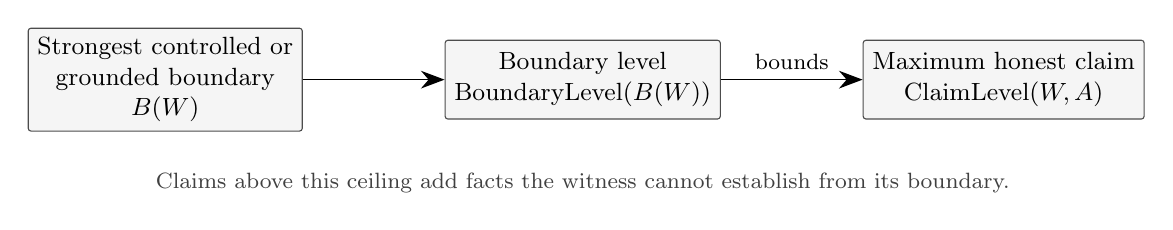
\begin{tikzpicture}[
  font=\small,
  box/.style={draw=black!70, rounded corners=1pt, minimum width=3.2cm, minimum height=1cm, align=center, fill=black!4},
  arrow/.style={-{Stealth[length=3mm]}, line width=0.6pt}
]
\node[box] (boundary) {Strongest controlled or\\grounded boundary\\$B(W)$};
\node[box, right=1.8cm of boundary] (level) {Boundary level\\$\mathrm{BoundaryLevel}(B(W))$};
\node[box, right=1.8cm of level] (claim) {Maximum honest claim\\$\mathrm{ClaimLevel}(W,A)$};
\draw[arrow] (boundary) -- (level);
\draw[arrow] (level) -- node[above, font=\footnotesize] {bounds} (claim);
\node[font=\footnotesize, align=center, text=black!75, below=0.55cm of level] {Claims above this ceiling add facts the witness cannot establish from its boundary.};
\end{tikzpicture}
}
\caption{Boundary Ceiling Principle as a claim-strength bound. The strongest execution-relevant boundary controlled or grounded by the witness determines the maximum honest execution-evidence claim. Independent verification qualifies a claim at its captured level and does not move this bound.}
\label{fig:boundary-ceiling-principle}
\end{figure}

\subsection{Status and Basis of the Axiom}
Version 1.0 presented this bound with a proof sketch that derived it from the definition of witnessability --- a circular derivation, since the definition already contains the bound. This revision states the commitment honestly: the $\mathrm{cap}$ assignment is an \emph{axiom} of the model, grounded in (not derived from) the operational definitions of Section 4 --- a witness that only observes an event has no access to facts requiring execution ownership; a witness that only records intent has no access to facts requiring invocation; a witness that mediates invocation has no access to the internal semantics of an execution it does not own. The corollaries of Section 6.3 are consequences of the axiom together with the cap assignment; they are not independent evidence for it. The axiom is falsifiable in the ordinary way for classificatory frameworks: by exhibiting a boundary type whose honest supportable claims systematically exceed its designated cap, which would force a revision of the assignment (Section 11).

\subsection{Corollaries}

\paragraph{Observation does not imply execution.} Seeing an event is not the same as owning the execution that produced it.

\paragraph{Intent does not imply invocation.} A recorded plan or approval does not prove that a call crossed a boundary.

\paragraph{Invocation does not imply execution ownership.} A mediated tool call does not prove the internal behavior of the invoked tool unless the witness owns that execution boundary or has grounded its record on it.

\paragraph{Execution ownership does not imply independent verification.} A runtime that owns execution may still be the sole producer and custodian of evidence.

\paragraph{Provenance does not imply runtime action.} A build attestation may prove how an artifact was produced, but not that a specific runtime action occurred.

\paragraph{Verifiability does not raise the captured level.} A verifiable record of an observation remains an observation; independent verification proves the record is genuine, not that a higher boundary was controlled.

\paragraph{System ceiling and event level differ.} A system may be capable of WL3 witnessability while a particular event only achieves WL1 or WL2 if execution results were not captured.

\medskip
\noindent These corollaries define the non-claims of each level --- what a record at a given execution-evidence level explicitly does not prove.

\subsection{Common False Inferences}

\begingroup
\setlength{\fboxsep}{8pt}
\noindent\fbox{%
\begin{minipage}{\dimexpr\textwidth-2\fboxsep-2\fboxrule\relax}
\textbf{Common false inferences.}
\begin{itemize}[leftmargin=*]
\item Observation $\neq$ Execution.
\item Intent $\neq$ Invocation.
\item Invocation $\neq$ Execution.
\item Execution $\neq$ Provenance.
\item Provenance $\neq$ Runtime Action.
\item Verification $\neq$ Higher Evidence Level.
\end{itemize}
\end{minipage}}
\endgroup

\section{Witness Boundary Taxonomy}

\subsection{Observation Boundaries}
Observation boundaries capture events without necessarily controlling their cause. Examples include logging agents, metrics collectors, tracing instrumentation, monitoring hooks, and event streams.

\subsection{Intent and Policy Boundaries}
Intent boundaries record plans, approvals, guardrail decisions, or policy evaluations. Examples include agent planning modules, policy engines, governance layers, approval workflows, and compliance controls.

\subsection{Invocation Boundaries}
Invocation boundaries mediate calls between actors and tools, services, APIs, or runtimes. Examples include API gateways, tool-calling protocols, MCP clients and servers, function routers, service proxies, and automation connectors.

\subsection{Execution Ownership Boundaries}
Execution ownership boundaries control actual execution. Examples include process runners, workflow activity workers, CI/CD runners, containers, sandboxes, serverless isolates, virtual machines, agent tool sandboxes, and secure enclaves.

\subsection{Provenance Boundaries}
Provenance boundaries link execution to origin, source, build, artifact, configuration, dependency, or deployment identity.

\subsection{Verification Boundaries}
Verification boundaries allow parties outside the original operator to validate evidence claims. Examples include third-party verifiers, transparency logs, public ledgers, reproducible builds, independent witness networks, external audit services, and remote attestation verifiers.

\section{Evaluation Method}
\label{sec:evaluation-method}

Each system is classified according to: (1) primary boundary controlled, (2) typical witnessability ceiling, (3) evidence artifacts, and (4) trust assumptions.

When a system supports multiple deployment modes, the classification uses a conservative default: a system is assigned the highest level generally attainable under its typical documented boundary, not the highest level attainable through custom integrations.

\section{Canonical Classification Examples}

The following examples illustrate how the model classifies common situations and where overclaims usually enter.

\subsection{AI Agent Invokes an External SaaS Tool}

\textbf{Claim.} An agent claims that an external SaaS tool executed a requested action.

\textbf{Evidence.} The agent runtime may record the planned action, tool name, request parameters, timestamp, and response.

\textbf{Boundary.} The agent controls the planning and invocation boundary, but the SaaS provider controls the tool's internal execution boundary.

\textbf{WL ceiling.} WL2 for the agent-side invocation record, unless the SaaS execution boundary is independently verified or the SaaS service returns stronger execution evidence.

\textbf{Common overclaim.} Treating a recorded tool call or returned message as proof that the remote tool executed internally as claimed.

\subsection{CI/CD Runner Executes a Build}

\textbf{Claim.} A CI/CD runner claims that it executed a build command and produced an artifact.

\textbf{Evidence.} The runner may record the command, environment, logs, exit code, artifact digest, and timestamps.

\textbf{Boundary.} The runner controls the process or job boundary in which the build executes.

\textbf{WL ceiling.} WL3 for owned execution evidence; WL4 if the execution is linked to source, artifact, or build provenance; WL5 only for the specific claim independently verified.

\textbf{Common overclaim.} Treating build provenance alone as proof of a later runtime action by the artifact.

\subsection{Distributed Tracing Observes a Request}

\textbf{Claim.} A tracing system claims that a request crossed a service boundary.

\textbf{Evidence.} Spans, timestamps, service names, request identifiers, latency, status codes, and correlated events.

\textbf{Boundary.} The tracing system observes or instruments request flow but may not own the execution environment that handled the request.

\textbf{WL ceiling.} WL0 for passive observation, rising toward WL2 only where the tracer controls or mediates the invocation boundary.

\textbf{Common overclaim.} Treating a trace of a request as proof that the requested action executed with the asserted internal semantics.

\subsection{Adversarial Example: Logged Tool Claim Without Execution}

\textbf{Claim.} An agent claims that a tool executed a side effect.

\textbf{Evidence.} The agent log contains a planned tool call and a record asserting success, but the tool never executed.

\textbf{Boundary.} If the agent only records its own plan or self-reported result, the evidence remains at the intent or observation boundary. If it controls a real outbound call boundary, it can support invocation, but not the tool's internal execution.

\textbf{WL ceiling.} WL1 for self-recorded intent, or WL2 if a controlled invocation actually crossed the tool boundary. It does not reach WL3 unless the witness owns the tool execution boundary or has grounded its record on it.

\textbf{Common overclaim.} Treating internally consistent logs as proof of external execution.

\section{Comparative Evaluation}

The classifications below are not product ratings or quality rankings; they indicate the typical evidence ceiling attainable under each system's documented boundary, consistent with the conservative default of Section~\ref{sec:evaluation-method}.

\begingroup
\footnotesize
\setlength{\tabcolsep}{3pt}
\renewcommand{\arraystretch}{1.12}
\begin{longtable}{@{}P{0.17\textwidth}P{0.22\textwidth}P{0.17\textwidth}P{0.14\textwidth}P{0.20\textwidth}@{}}
\toprule
Category & Example Systems & Primary Boundary & Typical Ceiling & Notes \\
\midrule
\endfirsthead
\toprule
Category & Example Systems & Primary Boundary & Typical Ceiling & Notes \\
\midrule
\endhead
Observability~\cite{opentelemetry_docs,opentelemetry_what_is} & OpenTelemetry, Jaeger, Prometheus & Observation & WL0--WL2 & Strong visibility; no inherent execution ownership. \\
Governance / Guardrails & Policy engines, guardrails & Intent / policy & WL1--WL2 & Records decisions and approvals; execution proof requires additional boundary. \\
Tool Protocols~\cite{mcp_intro,anthropic_mcp} & MCP-based systems & Invocation & WL2 & Mediates calls; tool execution depends on server/tool boundary. \\
Agent Frameworks~\cite{langgraph_persistence,autogen_repo,openai_agents_tracing} & LangGraph, AutoGen, OpenAI Agents SDK & Runtime-dependent & WL1--WL3 & Ceiling depends on whether framework owns tool execution or only orchestrates. \\
Workflow Engines~\cite{temporal_event_history,airflow_tasks} & Temporal, Airflow, Prefect, Dagster & Workflow / activity & WL2--WL3 & Stronger when activity execution is controlled. \\
CI/CD Platforms~\cite{github_actions_attestations,jenkins_durable_task} & GitHub Actions, Jenkins, GitLab CI & Runner / process & WL3--WL4 & Can execute commands and link to build provenance. \\
Automation Platforms~\cite{zapier_home,zapier_apps,n8n_executions,n8n_logging} & Zapier, Workato, n8n & Invocation / workflow & WL2--WL3 & SaaS integrations often cross external boundaries. \\
Serverless Runtimes~\cite{cloudflare_workers_how,cloudflare_workers_security} & Cloudflare Workers, Lambda-like systems & Isolate / runtime & WL3--WL4 & Strong execution boundary; provenance linkage depends on deployment evidence. \\
Coding Agents~\cite{openhands_platform_2024,agentforge_2026} & Claude Code, Cursor, OpenHands & Sandbox/tool runtime & WL2--WL3 & Stronger when execution occurs in owned sandbox. \\
Supply-Chain Attestation~\cite{slsa_provenance,intoto_attestation} & SLSA, in-toto, Sigstore & Provenance support & WL4--WL5 support & Strengthens provenance and verification, but does not itself own runtime action. \\
Trusted Execution~\cite{attestable_builds_2025,zk_compilation_2026,evidence_ci_2026} & TEEs, remote attestation & Measured environment & WL4--WL5 support & Can verify environment identity; still needs action-level evidence. \\
\bottomrule
\caption{Preliminary classification of contemporary systems.}
\end{longtable}
\endgroup

\section{Acceptance and Appraisal Semantics}
\label{sec:acceptance}

A verifier that evaluates a record against a claimed state produces a \emph{relation} between the claimed state and the verified state, under the componentwise order of Section~\ref{sec:qualified-states}:

\[
\mathrm{relation} \in \{\textsf{equal},\ \textsf{lower},\ \textsf{incomparable}\}.
\]

\paragraph{Acceptance.} A claim is \emph{accepted} exactly when one of the following holds:
\begin{enumerate}[leftmargin=*]
\item the verified state equals the claimed state;
\item the verified state exceeds the claimed state \emph{at the same content level} ($Q_{\mathrm{claimed}} \subseteq Q_{\mathrm{verified}}$, $\ell$ equal);
\item the verified content level is deeper than the claimed one \emph{and} the evidence satisfies the specific requirements of the claimed level.
\end{enumerate}
Clause 3 is restrictive by design: executional depth is not entailment. Evidence of execution does not, by itself, establish the existence of an approval; a claimed intent state is accepted from deeper evidence only where intent-level requirements (a bound plan, approval, or policy decision) are themselves satisfied. A claim that is neither accepted nor structurally invalid is \emph{unsupported as claimed}, with the relation (\textsf{lower} or \textsf{incomparable}) reported explicitly; ``incomparable'' is a first-class outcome, not an error.

\paragraph{Bottom outcome and limits.} Appraisal is total: where no content level's requirements are satisfied, the result is the bottom outcome \emph{no supported claim}, distinct from any WL0 claim. The result further distinguishes an \emph{evidence limit} (the record lacks the required evidence) from an \emph{evaluation limit} (the verifier lacks scope, trust context, or resolvable references to assess it); the two must not share a single failure token.

\paragraph{Counter-evidence.} Appraisal admits counter-evidence as input. An unresolved defeater that is material to the claimed state blocks acceptance of that state; the typed treatment of defeaters (rebutting, undercutting, undermining) follows the Conceptual Core~\cite{wcc_core_2026}.

\section{Composition of Segmented Claims}
\label{sec:composition}

An end-to-end action may cross several witnesses, each producing a record for its segment. Version 1.0 contained no composition rule; the numeric-minimum chain rule that circulated in early protocol work (draft-sergeev-wexp-core-00) is a protocol formulation, not part of Version 1.0, and it is corrected by this section.

\paragraph{Rule.} Let segments $S_1,\ldots,S_n$ have verified states $(\ell_i, Q_i)$. Composition is defined only under the \emph{binding precondition}: for each adjacent pair, binding evidence connects the segment records. Where defined, the state supportable for the chain is
\[
\Big(\min_i \ell_i,\ \bigcap_i Q_i\Big)
\]
subject to two qualifier preconditions:
\begin{itemize}[leftmargin=*]
\item \textbf{PROV survives} only if every $Q_i$ contains PROV \emph{and} the binding evidence covers the provenance linkage across segments;
\item \textbf{IV survives} only if every $Q_i$ contains IV, the binding evidence is itself independently verifiable, \emph{and} the verification roots of the segments are independent. Where roots are shared, IV is dropped and the reason is reported.
\end{itemize}

\paragraph{Two questions, two operations.} The rule above answers: \emph{what does the evidence support about the chain as a whole?} The distinct question --- \emph{what does it support about the terminal action?} --- keeps the terminal segment's content level where binding to the terminal action is established, and is otherwise undefined. Conflating the two questions under one formula was the source of divergent results in earlier material.

\paragraph{Algebraic properties.} Restricted to the $(\min, \cap)$ core (preconditions assumed satisfied), composition is the meet in the product of the chain $\mathrm{WL0}<\mathrm{WL1}<\mathrm{WL2}<\mathrm{WL3}$ with the Boolean lattice $2^{\{\mathrm{PROV},\mathrm{IV}\}}$.

\begin{quote}
\textbf{Lemma (closure).} The admissible state set is closed under componentwise meet. \emph{Proof.} Admissibility constrains only the pair structure: $\ell$ ranges over the four content levels and $Q$ over subsets, with $\mathrm{PROV} \in Q \Rightarrow \ell = \mathrm{WL3}$. If $\mathrm{PROV} \in \bigcap_i Q_i$ then $\mathrm{PROV} \in Q_i$ for all $i$, hence every $\ell_i = \mathrm{WL3}$ and $\min_i \ell_i = \mathrm{WL3}$. $\square$

\textbf{Corollary.} Composition is deterministic, associative, commutative, idempotent, and monotone in each argument, and is non-inflating componentwise: the composite never exceeds any segment in either component.
\end{quote}

Non-inflation of the \emph{composite claim} additionally requires the qualifier preconditions: intersection alone would preserve IV even where the inter-segment binding is not independently verifiable or the roots are shared, and the composite claim --- a different proposition from any segment claim --- would then overstate its verifiability. The preconditions, not the lattice algebra, carry that burden.

\paragraph{Shared test vectors.} The following vectors are normative for this model and for any protocol encoding it; a conforming verifier and this section must agree on all of them.

\begin{center}
\small
\begin{tabularx}{\textwidth}{@{}clY@{}}
\toprule
\# & Input & Expected result \\
\midrule
V1 & $(\mathrm{WL3},\{\mathrm{PROV}\}) \oplus (\mathrm{WL3},\{\mathrm{IV}\})$, binding ok, roots indep. & $(\mathrm{WL3}, \varnothing)$ --- not ``WL4''; a numeric minimum over labels would wrongly yield WL4 \\
V2 & claimed $(\mathrm{WL3},\{\mathrm{IV}\})$, capability ceiling truncates IV & re-derive attainable state; result $(\mathrm{WL3},\varnothing)$, never a state whose own requirements are unmet \\
V3 & $(\mathrm{WL3},\{\mathrm{IV}\}) \oplus (\mathrm{WL3},\{\mathrm{IV}\})$, shared verification root & $(\mathrm{WL3}, \varnothing)$, reason: shared root \\
V4 & self-recording tool runtime, claimed WL3, relation self-report & content WL3 only with the self-report qualification; no non-repudiation without recorder independence \\
V5 & two-record chain, non-genesis, binding via chained hash & composition defined; binding format fixed by test \\
V6 & $(\mathrm{WL2},\{\mathrm{IV}\}) \oplus (\mathrm{WL3},\varnothing)$, binding ok & $(\mathrm{WL2}, \varnothing)$; IV not inherited \\
\bottomrule
\end{tabularx}
\end{center}

\section{Migration and Display of Version 1.0 Labels}
\label{sec:migration}

Two distinct mappings connect Version 1.0's scalar labels to typed states; they must not be conflated.

\paragraph{Display projection (state $\to$ label).} Each state has exactly one canonical display (Section~\ref{sec:qualified-states}). The projection is lossy by design and is not invertible.

\paragraph{Semantic migration (legacy record $\to$ state).} A record produced under Version 1.0's cumulative reading asserted, at level $n$, all levels below $n$. Its faithful typed image is therefore:

\begin{center}
\small
\begin{tabularx}{\textwidth}{@{}llY@{}}
\toprule
Legacy label (cumulative era) & Typed state & Note \\
\midrule
WL0--WL3 & $(\mathrm{WL}n, \varnothing)$ & content level preserved; lower levels entailed by cumulativity \\
WL4 & $(\mathrm{WL3}, \{\mathrm{PROV}\})$ & \\
WL5 & $(\mathrm{WL3}, \{\mathrm{PROV}, \mathrm{IV}\})$ & cumulative-era WL5 included WL4's provenance; dropping PROV in migration would silently weaken the record's own claim \\
\bottomrule
\end{tabularx}
\end{center}

States $(\mathrm{WL0},\{\mathrm{IV}\})$, $(\mathrm{WL1},\{\mathrm{IV}\})$, and $(\mathrm{WL2},\{\mathrm{IV}\})$ have no legacy label; legacy records cannot have asserted them, and they arise only in new records. The migration table is exact for honestly produced legacy records; it is not a claim that such records were verified.

\section{Relation to the Witnessability Conceptual Core}
\label{sec:wcc-relation}

The Witnessability Conceptual Core~\cite{wcc_core_2026} defines Witnessability as a claim-relative capability over arbitrary Target Propositions. This model is a \emph{specialization} of that core to the execution class of Target Propositions: a witnessability state $(\ell, Q)$ is a profile-defined summary of a Support Envelope for execution propositions; a record is a constituent of a Witness Case (without the core's full argument structure); appraisal (Section~\ref{sec:acceptance}) is a constituent of a Support Assessment; and the evaluation profile of the verifier instantiates the core's Evaluation Profile, subject to the core's admissibility floor. Axiom BC is the execution-class instance of the core's non-amplification discipline; the core's Preservation Ceiling (DR-PC) is its conceptual generalization. Objects of the core deliberately outside this model's scope include the Relying-Party Decision, the Challenge Interface, and the full defeater typology (of which Section~\ref{sec:acceptance} adopts the acceptance-blocking discipline only). Appendix~A records the item-by-item Conceptual Consistency Mapping required by the core for any claim of alignment.

\section{Falsification Attempts and Edge Cases}

The model can be stress-tested by asking whether a system produces evidence not covered by WL0--WL5, controls a boundary not covered by the taxonomy, honestly claims execution evidence above its controlled boundary, achieves WL3 without execution ownership, or achieves WL5 without independent verification.

Current stress testing across contemporary systems suggests that systems map onto observation, intent, invocation, execution, provenance, or verification boundaries without requiring a new execution-evidence level. However, governance-decision recorders, physical-world actuation, remote attestation, and cross-boundary agent systems require further investigation.

\section{Discussion}

\subsection{Execution Ownership as Differentiator}
The evaluation suggests that execution ownership is the strongest differentiator among systems. Systems with many integrations may still only mediate invocation. Systems with fewer integrations but stronger runtime control may provide stronger witnessability.

\subsection{Governance Evidence vs Execution Evidence}
Governance evidence answers whether an action was allowed, intended, or compliant. Execution evidence answers what actually executed, under which boundary, with what result. A mature assurance architecture may require both.

\subsection{Observability vs Witnessability}
Observability answers what the system could see. Witnessability answers what the witness can honestly prove.

\subsection{Provenance vs Witnessability}
Provenance answers where an artifact, data item, or result came from. Witnessability asks what action can be proven about execution, and how that execution is linked to origin.

\subsection{Runtime Verification vs Witnessability}
Runtime verification answers whether an execution satisfies a property. Witnessability answers what kind of execution evidence exists for the verification to rely on.

\subsection{Why This Is Not Better Logging}
Logging is an artifact type. Witnessability is a claim-strength model. The same log record may support different execution-evidence levels depending on where it was produced, which boundary it crossed, and whether it is independently verifiable.

\section{Limitations}

This paper proposes a conceptual model and taxonomy, positioned alongside vendor-neutral assurance and provenance frameworks rather than as a systems contribution. It does not provide a performance benchmark, security proof, or empirical measurement of all surveyed systems. Systems vary by deployment mode, and the classification should be understood as a typical ceiling, not a universal judgment. Witnessability does not prove that an action was correct, safe, useful, ethical, or aligned with user intent. It only classifies what can be proven about the occurrence and evidence of execution. The model also bounds only what can be honestly claimed when evidence is produced; it does not by itself address evidence suppression---a witness or operator may withhold, omit, or decline to produce a record, and controlling a higher boundary does not compel a record to exist. Detecting or deterring such non-production lies outside the model and requires additional mechanisms such as mandatory logging, transparency requirements, or independent checks.

\section{Threats to Validity}

\paragraph{Compromised witnesses.} A compromised witness may produce false evidence or misrepresent the boundary it controls. The model classifies the claim a boundary can support under honest operation; it does not by itself prove that the witness was uncompromised.

\paragraph{Forged logs.} A log can be fabricated or altered. Forgery affects the integrity of the evidence artifact, while witnessability classifies the maximum claim the artifact could honestly support if authentic.

\paragraph{Withheld evidence.} A witness may omit evidence or decline to produce a record. Boundary control creates the ability to support a stronger claim; it does not guarantee that the evidence will be generated or disclosed.

\paragraph{Collusion.} Multiple parties may coordinate to present misleading evidence. Independent verification reduces some reliance on a single operator, but collusion remains an adversarial risk outside the level taxonomy itself.

\paragraph{Ambiguous boundaries.} Some systems blur observation, invocation, and execution ownership, especially when responsibility is split across hosted services and plugins. Such cases should be classified conservatively unless the controlled boundary is explicit.

\section{Future Work}

Future work should refine methods for identifying execution-relevant boundaries, study physical-world actuation and cross-domain runtime settings, and examine how independent verification mechanisms vary across deployment contexts. Further work may also test whether the WL0--WL5 taxonomy remains stable across additional classes of AI and software execution systems.

\section{Conclusion}

Modern AI and software systems produce many forms of evidence, but these artifacts are often conflated. Logs, traces, approvals, attestations, workflow histories, and verification reports do not all prove the same thing.

This paper introduced the Witnessability Model, a boundary-based framework for classifying the strength of execution-related evidence. The model distinguishes observation, intent, invocation, execution, provenance linkage, and independent verification. The central result is the Boundary Ceiling Principle: $\mathrm{ClaimLevel}(W,A) \leq \mathrm{BoundaryLevel}(B(W))$. A witness cannot honestly claim evidence above the boundary it controls or has grounded its record on; independent verification qualifies a claim at its captured level rather than raising it.

The comparative evaluation suggests that execution ownership, rather than integration breadth or policy sophistication, is the primary determinant of attainable witnessability. Witnessability provides a vocabulary for reasoning about execution evidence independently of any specific product, vendor, or implementation.

\section*{Author Note}

\noindent\textbf{Disclosure:} One author, Mikhail A. Sergeev, has a commercial interest in execution-evidence and runtime-assurance tooling. This paper presents a vendor-neutral conceptual model and does not describe, evaluate, or endorse any specific proprietary implementation.

\appendix
\section{Conceptual Consistency Mapping (WCC 1.1)}
\label{app:ccm}

Mapping against checklist items CCM-1--CCM-18 of the Witnessability Conceptual Core 1.1~\cite{wcc_core_2026}. Bound versions: Core 1.1; this model 1.1. ``Deferred to profile'' marks obligations this conceptual model assigns to evaluation profiles and protocol encodings rather than discharging itself.

\begin{center}
\footnotesize
\begin{tabular}{@{}lp{10.2cm}@{}}
\toprule
Item & Treatment \\
\midrule
CCM-1 & Execution-class Target Propositions typed by the claim grammar (Section 4.2): actor, action, boundary, time, input, output, environment, origin, verifier, trust assumptions. \\
CCM-2 & Record $\subset$ Witness Case; appraisal $\subset$ Support Assessment; verifier profile = Evaluation Profile; Relying-Party Decision out of scope (Section~\ref{sec:wcc-relation}). \\
CCM-3 & Grounding defined (Section 4); full argument-graph representation deferred to profile. \\
CCM-4 & System ceiling vs.\ achieved event level (Section 4.1) preserves the configured/realized distinction. \\
CCM-5 & Binding evidence required for composition and terminal-action claims (Sections 4, \ref{sec:composition}). \\
CCM-6 & Partially: capture-coverage accountability deferred to profile; the model contributes the boundary-relative ceiling on what captured evidence can support. \\
CCM-7 & PROV qualifier requires bound origin linkage; provenance-chain reconstruction deferred to profile. \\
CCM-8 & Verified states are relative to verifier trust context; evaluation context is a mandatory component of results (Section~\ref{sec:acceptance}). \\
CCM-9 & Axiom BC; non-inflating composition with explicit preconditions (Sections~\ref{sec:axiom-bc}, \ref{sec:composition}). \\
CCM-10 & Bottom outcome; evidence-limit vs.\ evaluation-limit; incomparable as first-class relation (Section~\ref{sec:acceptance}). \\
CCM-11 & Witness Boundary Taxonomy with designated caps (Sections 7, \ref{sec:axiom-bc}). \\
CCM-12 & Deferred to profile; the model requires profile identity in evaluation context. \\
CCM-13 & Display projections declared profile-relative; scalar presentation never used as verdict arithmetic (Section~\ref{sec:qualified-states}). \\
CCM-14 & Reliance decisions out of scope by construction; verdicts are bounded support statements, not action policies. \\
CCM-15 & Trust roots and grounding assumptions are terminal dependencies; root independence explicit in composition (Section~\ref{sec:composition}). \\
CCM-16 & Not applicable: the execution class contains no normative Target Propositions; compliance mappings over this model must supply their own normative bridge. \\
CCM-17 & Not applicable at model level: non-occurrence propositions are outside the execution claim grammar; profiles adding them inherit the core's discipline directly. \\
CCM-18 & Shared verification roots collapse IV in composition; identifier distinctness insufficient; aliasing carried as qualification (Section~\ref{sec:composition}). \\
\bottomrule
\end{tabular}
\end{center}

\printbibliography

\end{document}
